% !TEX root =  ../../master.tex
\subsection{Grundgerüst}

Um auf den einzelnen Unterseiten der Anwendung einen allgemeinen und jeweils gleichen Anhaltspunkt zu besitzen, wird das Grundgerüst, welches in Abbildung \ref{fig:MockGrundgeruest} dargestellt ist, verwendet.
In diesem wird eine grundlegende Struktur festgelegt, welche einheitlich auf den Unterseiten der Webanwendung verwendet werden soll.
Dies soll dazu führen, dass die Benutzer schnell eine Vertrautheit mit der Seite erlangen.
Dabei wird die Seite in unterschiedliche Sektoren untergliedert.
Die einzelnen Komponenten einer Seite sind dabei der \emph{Header}, der \emph{Inhalt der Seite}, sowie der \emph{Footer}.
Wie schon die Namen der Sektoren indizieren, ist die Anordnung von \emph{Header} über den \emph{Inhalt der Seite} zu dem abschließenden \emph{Footer}, strukturiert.
Jedoch besitzen diese Komponenten im Mock-Up nicht die maximale Breite.
Daher gibt es an den rechten und linken Rand der Seite jeweils ungenutzte Flächen.
Diese freie Flächen sind jedoch gewollt, dadurch soll der Benutzer nicht durch eine zu große Menge an Informationen überfordert werden, wodurch seine Aufmerksamkeit auf den dargestellten \emph{Inhalt der Seite} gelenkt werden soll.

\begin{figure}[H]
	\centering
	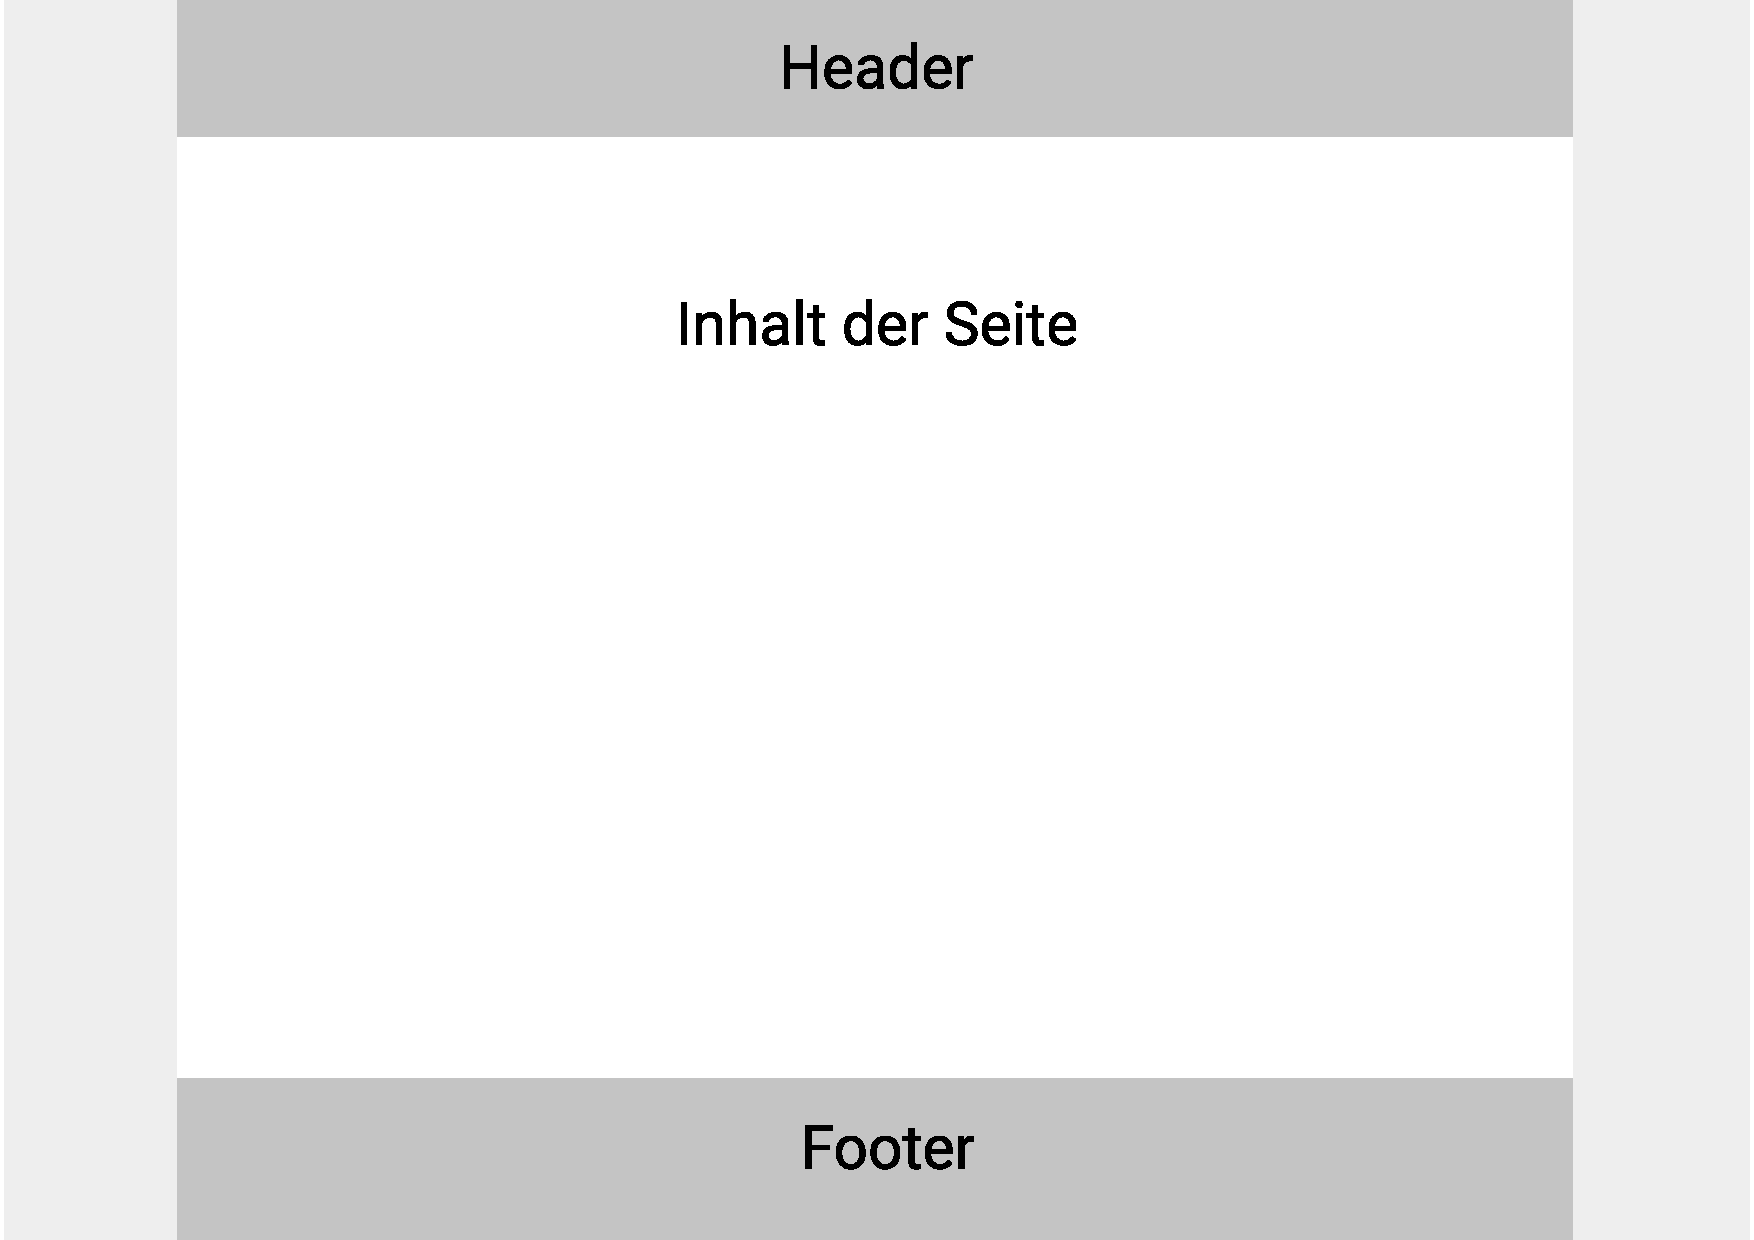
\includegraphics[width=0.7\textwidth]{img/konzeption/client/grundgeruest}
	\captionsetup{justification=centering, format=plain}
	\caption[Mock-Up vom Grundgerüst der Anwendung]{Mock-Up vom Grundgerüst der Anwendung \\\figma}
	\label{fig:MockGrundgeruest}
\end{figure}
